\lab{Monte-Carlo Integration}{Monte-Carlo Integration}
\objective{Use Monte-Carlo integration to estimate areas.}

Integration is important in a variety of applications. 
However, high-dimensional integration is highly inefficient using the standard one-dimensional methods. 
Accordingly, we are forced to pursue a different method. 
The method of choice in high dimensional settings is known as Monte-Carlo Integration, and is based upon random sampling. 
This technique is applied in a large variety of fields, such as optimization, physics, and finance.

Consider the following example: Suppose our goal is to estimate the area of a circle (we select this problem because it has a closed form solution, which we can use to test the method). 
One method that we could use for empirically finding that area is to throw darts randomly at a square board.
We then can find the area of the circle by multiplying the square's area by the percentage of darts that fell in the inscribed circle. 
We can do this using the following code (the resulting figure is shown in Figure \ref{Fig:MCCircle}).

\begin{lstlisting}
import numpy as np
points = np.random.rand(2, 500).T
points = 4*(points-.5)
pointsNorm = np.hypot(points[:,0],points[:,1]) <= 1
InCircle = points[pointsNorm]
OutCircle = points[~pointsNorm]
plt.plot(InCircle[:,0], InCircle[:,1], 'r.')
plt.plot(OutCircle[:,0], OutCircle[:,1], 'b.')

# Plot the circle
theta = np.linspace(0, 2*np.pi, 50)
plt.plot(np.cos(theta), np.sin(theta),'k')

plt.axis('equal')
plt.axis([-2, 2, -2, 2])
plt.show()

area = 4.0*InCircle.size/numPoints
\end{lstlisting}

\begin{figure}
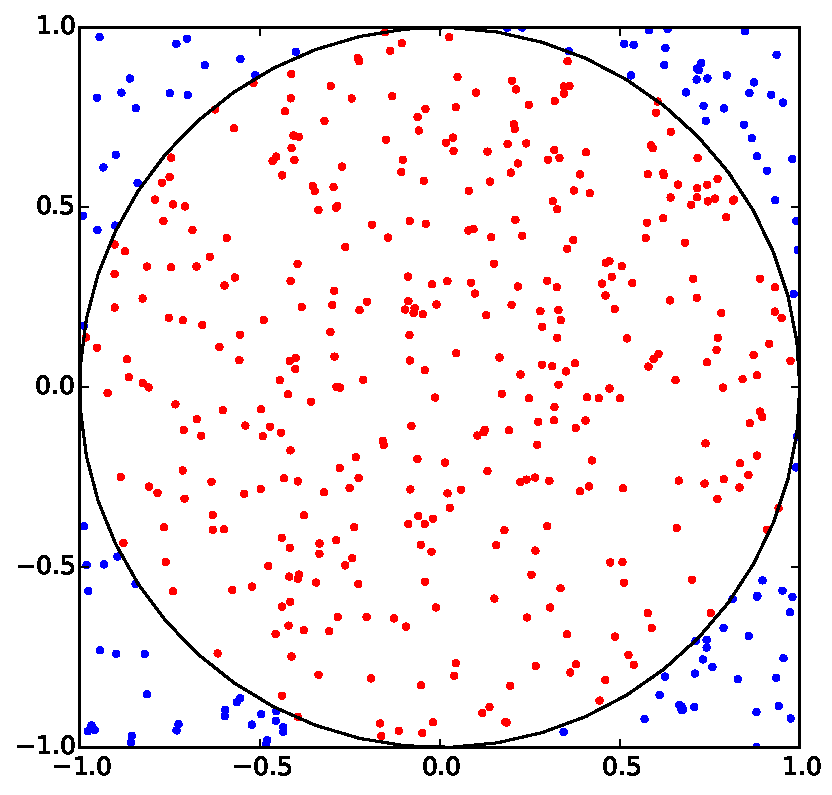
\includegraphics[width=\textwidth]{MC_Circle.pdf}
\caption{Finding the area of a circle using random points}
\label{fig:MCCircle}
\end{figure}

In this case the area should be $\pi$, and the approximation is pretty good.

One important question is the rate at which our estimate converges. 
We can test this using a log plot using the following code:
\begin{lstlisting}
numTestPoints = 29
testPoints = np.around(np.linspace(1000,100000,numTestPoints))
error = np.zeros(testPoints.size)
testRuns=100
area = np.zeros(testRuns)

for i in range(0,numTestPoints):
	for k in range(0,testRuns):
		numPoints = testPoints[i]
		points = np.random.rand(numPoints,2)
		points = 2*(points-.5)
		pointsNorm = np.hypot(points[:,0],points[:,1])
		inCircle = np.count_nonzero(pointsNorm < 1)
		area[k] = 4.0*inCircle/numPoints
	error[i] = np.mean(np.absolute(area-sp.pi))
error.size
testPoints.size

plt.loglog(testPoints, error)
estimate = la.lstsq(np.vstack((np.log(testPoints),np.ones(testPoints.size))).T, np.log(error))
convergenceRate = estimate[0][0]
\end{lstlisting}

Note that we estimate the convergence rate using Least Squares, as in Lab \ref{Stats1}. 
The rate should be something like $-.5$. 
This means that the estimate of the error improves as $1/\sqrt{N}$, meaning that to improve our error estimate by 10 times (one digit) we must sample 100 times more points. 
This is not a very desirable convergence rate. 
However, this rate is independent of the number of dimensions (a property not shared by one-dimensional integration techniques), and is therefore desirable for high-dimensional problems.

The problem of calculating the area of a circle above can actually be reformulated as the following integration problem:
\[
\mbox{Estimate }A = \int_{[-1,1]\times[-1,1]} f(x,y) dA
\]
where
\[
f(x,y) = \begin{cases} 1 &\mbox{ if $x$,$y$ is in the unit circle} \\ 0 &\mbox{ otherwise} \end{cases}
\]

Using a similar method we can actually solve any integration problem. 
Suppose that we desire to solve the integral
\[
\int_\Omega f(x) dV
\]

Where $\Omega$ is a region and $x \in \Omega$ is a vector. 
We can approximate the integral using the formula
\[
\int_\Omega f(x) dV \approx V(\Omega) \frac{1}{N} \sum_{i=1}^N f(x_i)
\]

Where $x_i$ are uniformly distributed random vectors in $\Omega$, and $V$ gives the volume of a region. 
This formula exactly describes how to perform Monte Carlo Integration. 
Now the intuition behind this formula is that $\frac{1}{N} \sum_{i=1}^N f(x_i)$ is the average value that $f$ obtains over $\Omega$ then we multiply that average value by the volume of $\Omega$ to get the integral.

As an 1-d example take the integral 
\[
\int_0^1 x dx \approx (1-0)\frac{1}{N} \sum_{i=1}^N x_i=\frac{1}{N} \sum_{i=1}^N x_i
\]

It is easy to see that the answer to the exact integral on the left-hand-side is $1/2$. 
In the approximation on the right-hand-side, the volume of the domain in $1$ and then $x_i$ is draws from a uniform distribution between zero to one. 
The average of $N$ draws will quickly converge to $1/2$. 

\begin{problem}
\label{prob:mc}
Write code implementing Monte Carlo Integration on a box of arbitrary number of dimensions for an arbitrary input function. 
Require the user to input the function and the bounds of the box. 
You may require that the user input the number of dimensions. 
Allow the user to input the number of points to use as well.
\end{problem}

\begin{problem}
\label{prob:mc_test}
Test your solution to Problem \ref{prob:mc}, and the convergence of the method, on the function:
\[
f(w,x,y,z) = sin(x) y^5 -y^3 + zw + yz^3
\]
Over the unit square of dimension 4 (with bounds from -1 to 1). 
This integral should converge to zero. Graph the error for N= 10,100,1000,10000.
\end{problem}

One application of Monte Carlo integration is integrating probability density that do not have a closed form solutions.

\begin{problem}
The standard normal distribution is an important object of study in probability and statistic.
It is defined by the density function $\frac{1}{\sqrt{2 \pi}} e^{- \frac{x^2}{2}}$.
(Here we are assuming a mean of $0$ and a variance of $1$).
This is a function that cannot be integrated symbolically.
We can use monte carlo integration to estimate the probability that a normally distributed random variable will take a value below a given point.
The probability that the random variable we are considering is less than (or equal to) a given value $x$ is
\[\int_{-\infty}^x \frac{1}{\sqrt{2 \pi}} e^{- \frac{t^2}{2}} dt\]
This function is essentially zero for values of $x$ that lie reasonably far from the mean, so we can estimate this probability by integrating from $-5$ to $x$ instead.

Compare your result at $x = 1$ with the output of the code
\begin{lstlisting}
from scipy.stats import norm
N = norm()
N.cdf(1)
\end{lstlisting}
\end{problem}

\begin{problem}
The joint normal distribution is an important object of study in probability and statistic. 
If $\bold{x} \in \mathbb{R}^k$ and the $x_i$ are independent from each other with mean $0$, variance $1$. 
The joint density function is defined by $\frac{1}{\sqrt{(2 \pi)^k}} e^{- \frac{\bold{x}^T\bold{x}}{2}}$.
This is a function that can not be integrated symbolically.
We can use Monte Carlo integration to estimate the probability the values are in a certain range.
The probability that the random vector is in a certain range is
\[
\int_{\Omega} \frac{1}{\sqrt{(2 \pi)^k}} e^{- \frac{\bold{x}^T\bold{x}}{2}}
\]
where $\Omega$ is the box you are integrating over.
Have you function take in the bounds and the number of dimensions and output the value of the integral.

\end{problem}

We note that we must use caution in using Monte Carlo integration when we don't know if the integral actually converges to a finite value. 
For example the following integral does not converge(is not finite):
\[
\int_0^1 \frac{1}{x}
\]

We can attempt Monte Carlo Integration on such an integrand using the following code:
\begin{lstlisting}
k = 5000
np.mean(1/np.random.rand(k,1))
\end{lstlisting}

We will get a finite value in return, so we could assume (incorrectly) that this integral has a finite value.
However, by experimenting with larger values of $k$ you will notice that the integral does not converge to a specific value, which is because the actual integral does not converge. 
Therefore it is often important to understand some of the properties of the integrand analytically prior to using this type of integration.

Another important key to successful Monte Carlo integration are that the random numbers be uniformly distributed. 
If they are not, our answer will not converge to a correct answer. 
This is one of the reason that good pseudo-random number generators are so important.

\begin{comment}
\begin{problem}
\label{prob:mc_flawed}
Create a new function (based upon the function from Problem \ref{prob:mc}) that uses a ``flawed'' random number generator that doesn't produce numbers between $-.95$ and $-1$. Test your method on the function from Problem \ref{prob:mc_test}. How bad is the error? 
\end{problem}
\end{comment}
